
Este capítulo oferece o arcabouço teórico necessário para a compreensão da pesquisa em si. 
Portanto, serão abordados conceitos fundamentais relacionados
a criptomoedas, \textit{blockchain}, RNAs, ARIMA e previsão em séries temporais.
\section{Bitcoin}
\label{secao:bitcoin}

A ideia de ativos digitais descentralizados baseados em criptografia, ou criptomoedas, foi marcada por inúmeras tentativas anteriores; contudo,
só foi implementada com o advento da \textit{Blockchain} \cite{Moi}. Além disso, é referida por \textcite{Yuan} como um registro compartilhado distribuído, no qual a verificação, o armazenamento, a manutenção e a transmissão dos dados são baseados na confiança mútua entre as partes, estabelecida por meio de algoritmos matemáticos.
Tal estrutura é formada por blocos que contêm um conjunto 
de transações, sendo que cada um possui um identificador exclusivo chamado \textit{Hash},
gerado a partir das informações presentes no bloco, incluindo as do anterior. 
Esse encadeamento de blocos cria uma sequência contínua e cronológica na qual os blocos são ligados ao anterior, formando uma cadeia \cite{Blockchain}.

\begin{figure}[!htb] \centering
  \caption{Representação da Blockchain} \label{figura:imageBlock}
  \begin{varwidth}{\linewidth}
    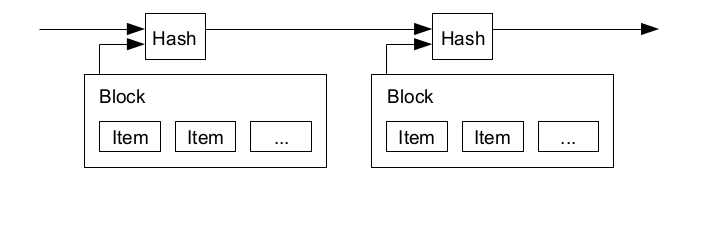
\includegraphics[width=8cm]{figuras/imageBlock.png}
    \fonte{\citefonte{Nakamoto}.}
  \end{varwidth}
\end{figure}

Segundo \textcite{Fer}, o primeiro e mais conhecido ativo desse setor se chama Bitcoin, definido como um dinheiro eletrônico negociado diretamente entre pares, sem passar por uma instituição financeira \cite{Nakamoto}.
Desde então, tem sido publicados diversos artigos que buscam explorar essa nova área de mercado. Segundo \textcite{Sousa}, as tecnologias baseadas em \textit{Blockchain} são mais rápidas, ágeis e seguras que seus pares centralizados. 
Por isso, esse nicho vem ganhando bastante espaço na mídia, atraindo, assim, interesse por parte de investidores individuais e fundos \cite{Yuan}. 

Cada \textit{Bitcoin} é subdividido em 100 milhões de unidades menores chamadas Satoshis, ou, simplesmente, "Sats".
Seu armazenamento é feito em uma carteira digital ciptografada de maneira assimétrica \textit{Offline}, chamada \textit{Cold Wallets}, ou \textit{Online}, em serviços de \textit{Hot Wallets} \cite{wallet}.
A transferência ocorre por prova de trabalho; um validador chamado de minerador é responsável por resolver um problema matemático de dificuldade variável. Além disso, serve como nó que confere a operação de outros mineradores e garante a integridade da rede.
Quando o problema é resolvido, adiciona-se um bloco de transação na \textit{Blockchain}; em troca, o minerador recebe uma recompensa em \textit{Bitcoins} \cite{pow}.
A dificuldade da prova de trabalho é ajustada automaticamente pelo \textit{Hashrate}, indicador que mede a quantidade de poder computacional necessário à mineração. Quanto maior o \textit{Hashrate}, mais difícil é encontrar o próximo bloco, regulando o tempo entre a adição de novos blocos à rede, mantendo uma média de 10 minutos.

\begin{figure}[!htb] \centering
    \caption{Prova de trabalho} \label{figura:imageNonce}
    \begin{varwidth}{\linewidth}
      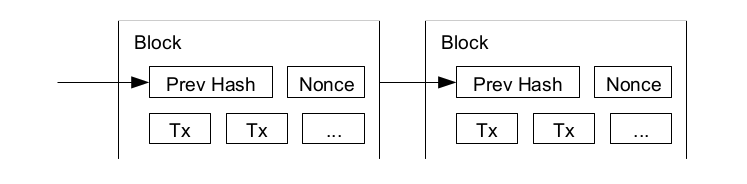
\includegraphics[width=8cm]{figuras/nonce.png}
      \fonte{\citefonte{Nakamoto}.}
    \end{varwidth}
  \end{figure}

A cada quatro anos, o número de \textit{Bitcoins} gerados por bloco é reduzido pela metade, evento conhecido como \textit{Halving}.
O fator de redução confere à moeda uma escassez programada, limitada a 21 milhões de unidades, que a torna deflacionária.
Ativos baseados em criptografia e a inteligência artificial são parte fundamental da \textit{Web 3.0}, considerada como a terceira geração da internet \cite{web3}.
Recentemente, os contratos inteligentes, \textit{DeFi} (Finanças Descentralizadas), \textit{NFTs} (Tokens Não Fungíveis) e a inteligência artificial generativa ensaiam uma nova era de aplicações e serviços \cite{books}.

\begin{figure}[!htb] \centering
    \caption{Livros lançados por assunto} \label{figura:imagengram}
    \begin{varwidth}{\linewidth}
      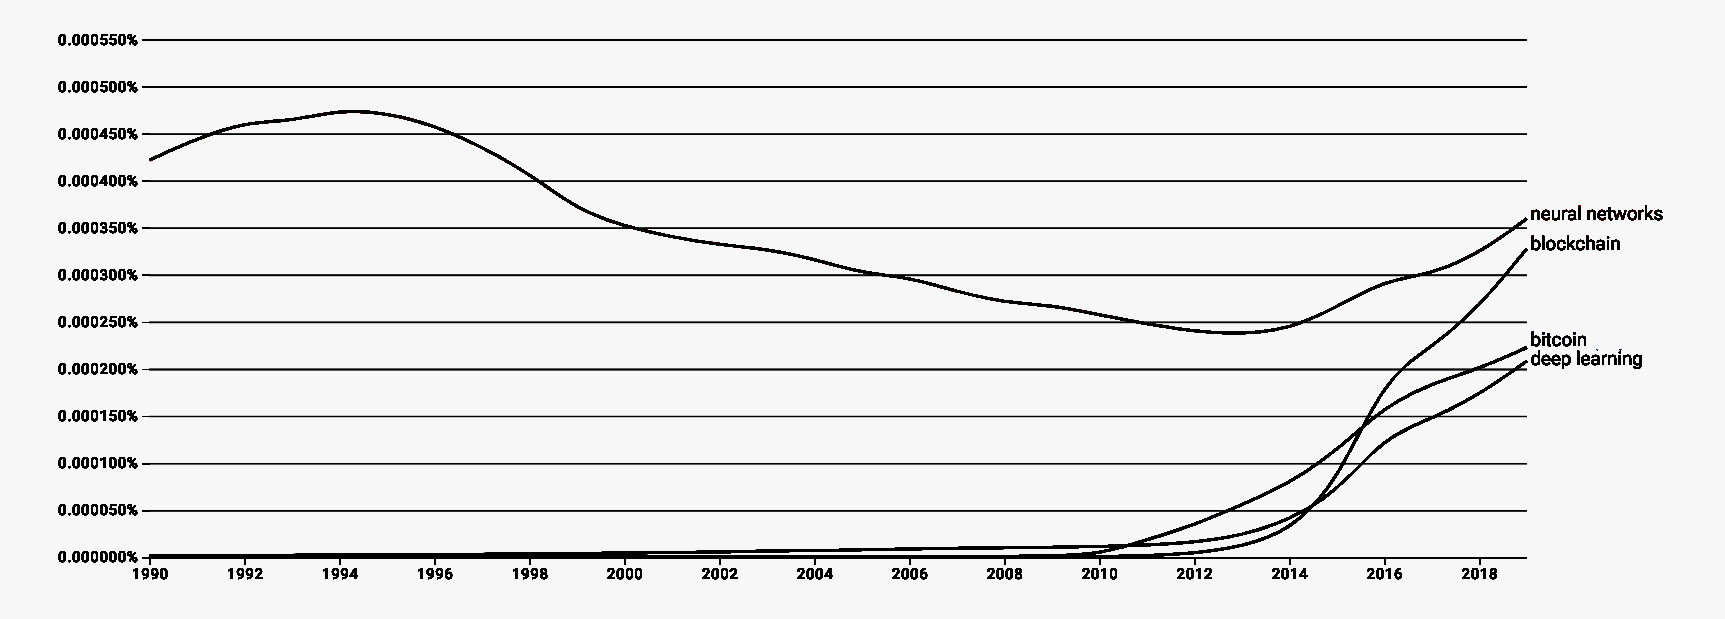
\includegraphics[width=15cm]{figuras/ngram.png}
      \fonte{\cite{books}}
    \end{varwidth}
  \end{figure}

No contexto de negociação do \textit{Bitcoin}, a mais conhecida das \textit{Exchanges} é a Binance, que opera em diversos países e possui um volume de transações diário de bilhões de dólares \cite{FakeExchanges}.
Com uma liquidez alta, o \textit{Spread}, diferença entre o preço de compra e venda, é baixo, o que representa o valor bem acurado com o oferecido no mercado.
Além disso, existem \textit{sites} de comparação de preços, sendo os mais populares o CoinGecko e CoinMarketCap, funcionando
como portais que classificam as plataformas, moedas e até a situação atual do mercado, por meio de índices, como visto na Tabela \ref{tabela:lista_produtos}.


% em 29 de jun. 2024
\begin{table}[!htb]
  \caption{Exchanges com maior volume e confiabilidade} \label{tabela:lista_produtos}
  \begin{tabularx}{\textwidth}{l|c|c|c} \hline
    Exchange      & Volume 24h (BTC) & Score Coingecko & Score CoinMarketCap  \\ \hline
    Binance (Global)      & 135.157      & 10/10        & 9,9/10 \\
    Bybit         & 44.720      & 10/10        & 7.6/10  \\
    HTX (Huobi)       & 34.250     & 9/10        & 6.9/10  \\ \hline
  \end{tabularx}
  \fonte{Elaborado pelo autor, 2024.}
\end{table}

%\section{\textit{Aprendizado de máquina}} \label{sec:apc}

\section{\textit{Autoregressive Integrated Moving Average}} \label{sec:arima}

O ARIMA (\textit{Autoregressive Integrated Moving Average}) tem suas raízes na econometria e na estatística.
Sua história remonta ao trabalho de \textcite{Box}, no qual os autores introduziram uma abordagem sistemática para identificar, estimar e diagnosticar modelos de séries temporais, conhecida como metodologia Box-Jenkins \cite{Arima}.
Combina três componentes principais: autorregressão (AR), diferenciação (I) e médias móveis (MA) - A componente; AR descreve a relação entre uma observação atual e observações passadas; e a componente MA modela a dependência entre uma observação e erros de previsão passados. 

Então, atribui-se a cada uma das componentes do modelo as siglas \textit{p}, \textit{d} e \textit{q}, representando o ajuste na série. O parâmetro \textit{p} é a ordem do modelo AR, \textit{d} é o grau de diferenciação (I) e \textit{q} é a ordem do modelo MA.
Para ajustar o modelo aos dados, o comum é usar uma análise das funções de autocorrelação total e parcial (ACF e PACF) ou a grade de busca (\textit{grid search}) com validação cruzada para otimizar esses valores, minimizando o erro.
Existem outras variantes dos métodos ARIMA, como o SARIMA (ARIMA sazonal) e o SARIMAX (ARIMA sazonal com variáveis exógenas).
\section{Redes neurais artificiais} \label{sec:redes neurais}

A teoria das redes neurais artificiais (RNAs), do inglês \textit{Artificial neural networks} (ANNs), surgiu com os estudos realizados por \textcite{Rosenblatt}.
Este autor desenvolveu o \textit{Perceptron}, um algoritmo fundamentado nas teorias formuladas por \textcite{McCulloch, hebb}, que modelavam as conexões dos neurônios no cérebro de animais \cite{Good}.
Apesar de suas vantagens, à época, o \textit{Perceptron} era capaz de resolver apenas problemas linearmente separáveis, como destacado por \textcite{Minsky}. Este fato o impedia de ser utilizado em muitos problemas reais,
o que causou uma crise no estudo da área como um todo, fato que mais tarde foi contornado por \textcite{Rumelhart}, que, juntos, desenvolveram o algoritmo de \textit{Backpropagation} para treinar a arquitetura denominanda \textit{Multilayer Perceptron} (MLP).

\begin{figure}[!htb] \centering
  \caption{Camadas de uma MLP} \label{figura:multilayer}
  \begin{varwidth}{\linewidth}
    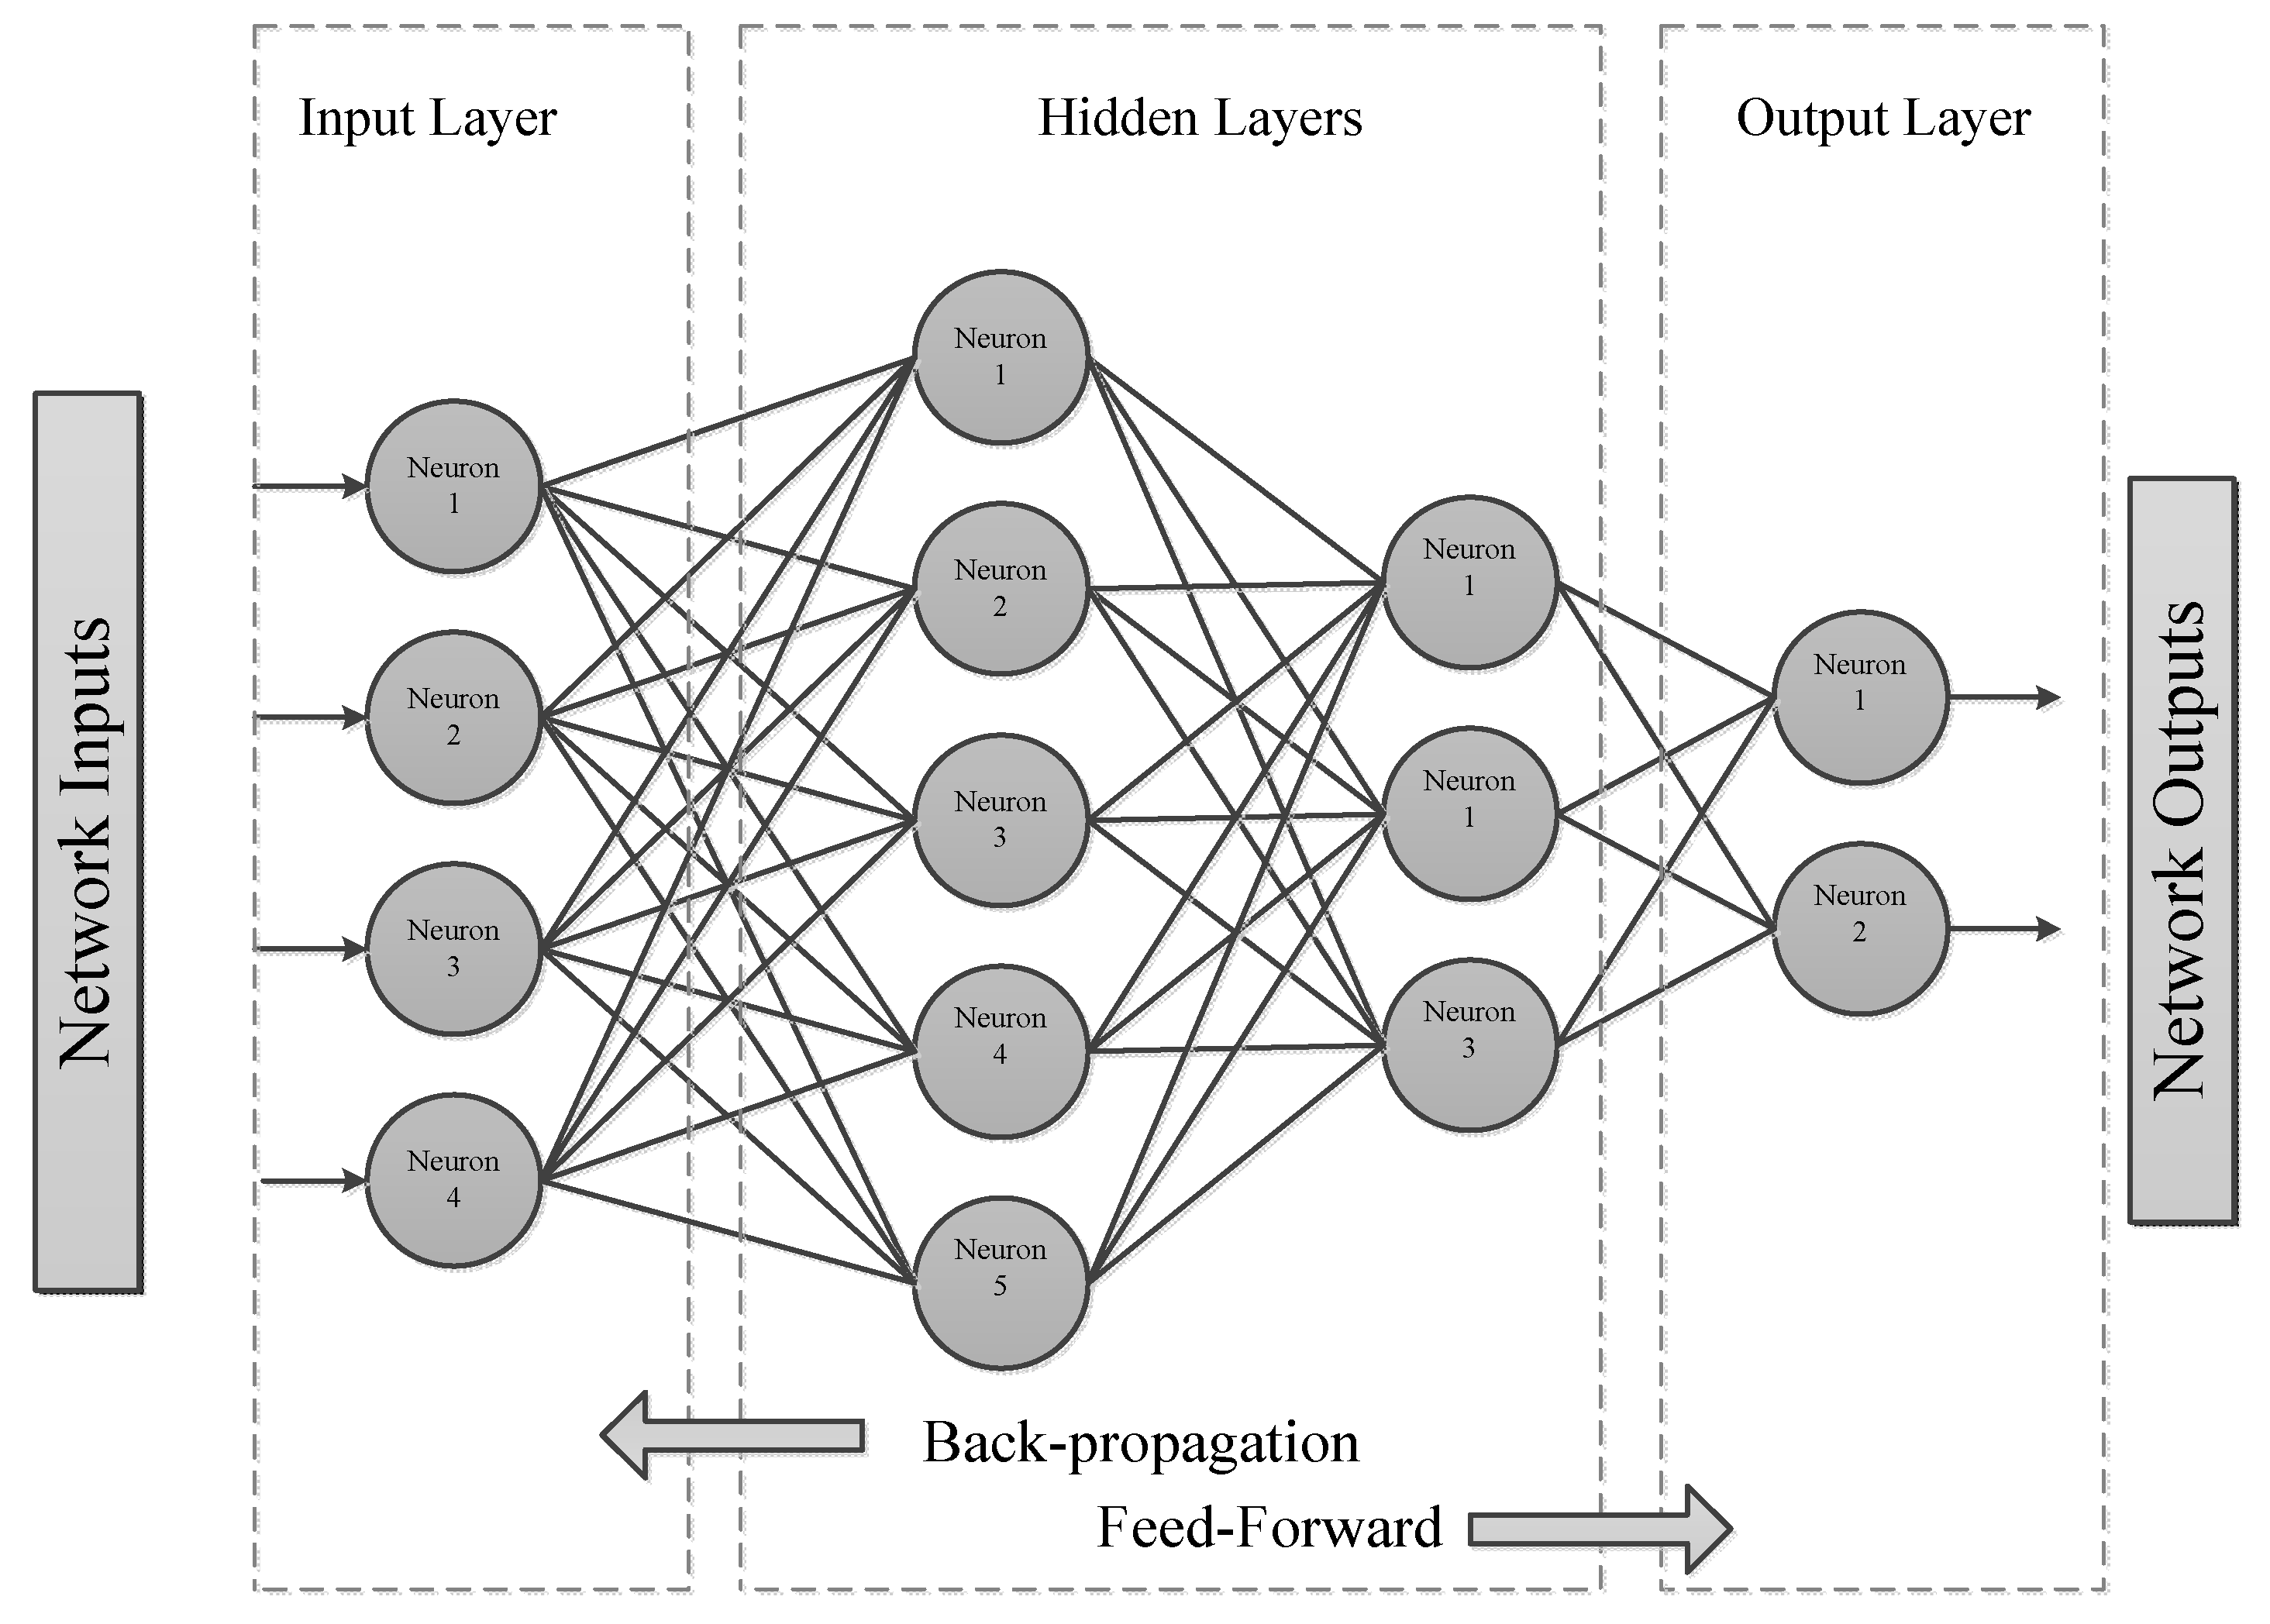
\includegraphics[width=12cm]{figuras/mlp.png}
    \fonte{\cite{multilayer}}
  \end{varwidth}
\end{figure}

Após esse início, os algoritmos baseados em RNAs evoluíram de forma a se tornar cada vez mais precisos e especializados em tarefas distintas.
Pode-se dar destaque neste contexto aos modelos
que podem ser combinados para gerar arquiteturas no que hoje é conhecido como \textit{Deep Neural Networks} (DNNs) ou \textit{Deep Learning} \cite{Good}. 
Como se verifica nas revisões bibliográficas mais recentes, tais modelos vêm demonstrando grande capacidade de auxiliar na resolução de problemas de classificação, previsão e análise de sentimentos \cite{Hanc}.

\subsection{\textit{Recurrent Neural Networks}} \label{sec:rnn}

Das arquiteturas apresentadas, é possível notar que representam grafos cujas arestas não formam ciclos na mesma fase.
Quando tal condição é subvertida e se estabelecem ciclos, como visto na Figura \ref{figura:rnn}, obtêm-se redes neurais recorrentes (RNRs), do inglês \textit{Recurrent Neural Networks} (RNNs)\cite{graves}.
Embora essa diferença possa parecer trivial, as implicações devem ser consideradas na implementação.
Enquanto uma MLP percorre apenas entre vetores de entrada e saída, \textcite{graves} destaca que uma RNN, a princípio, consegue mapear todo o histórico de entradas para cada saída, atuando como uma memória que persiste de resultados passados para execuções futuras. 
Pode-se, então, inferir a utilidade desses modelos em dados sequenciais $x^{(1)}$, ..., $x^{(\tau)}$ \cite{Good}.

\begin{figure}[!htb] \centering
  \caption{Camadas cíclicas de uma RNN} \label{figura:rnn}
  \begin{varwidth}{\linewidth}
    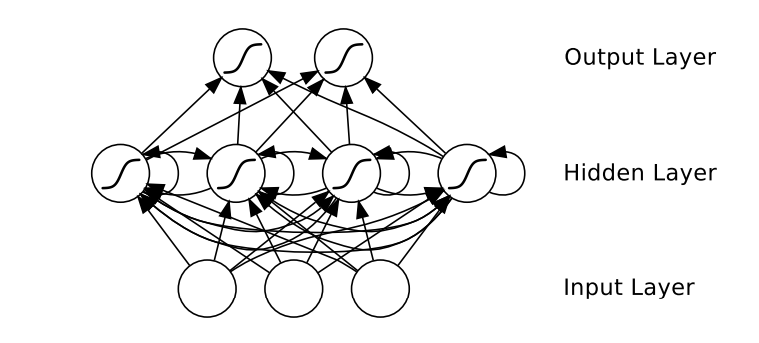
\includegraphics[width=12cm]{figuras/rnn.png}
    \fonte{\cite{graves}}
  \end{varwidth}
\end{figure}

Armazenar dependências ao longo das iterações é certamente o principal desafio matemático na implementação de redes recorrentes.
Segundo \cite{graves}, o problema consiste no fato de que gradientes propagados por muitas execuções tendem a desaparecer (na maioria dos casos) ou explodir (raramente, mas com grande impacto na otimização).
Mesmo assumindo que os parâmetros da rede sejam estáveis, a dificuldade surge à medida que o modelo converge ao passar das épocas e os 
\textit{Steps\footnote{ O salto no aprendizado (ou \textit{step}) da rede se tornar exponencialmente menor pode ser explicado observando as mínimas ou máximas locais e globais em uma função n-dimensional. Fato demonstrado no livro de \textcite{stewart}.}} 
se tornam cada vez menores \cite{Good}.
Uma maneira de lidar com a dispersão dos gradientes é projetar um modelo que opere em múltiplas escalas temporais \cite{Bengio} e realizar o 
\textit{Clipping\footnote{\textit{Clipping} é uma técnica que consiste em limitar a magnitude dos gradientes a um intervalo válido, impedindo que ultrpassem valores predefinidos.}} dos gradientes, para evitar as explosões \cite{Exp}.

\subsection{\textit{Long-Short Term Memory}} \label{sec:lstm}
Os modelos baseados em células de memória \textit{Long-Short Term Memory} (LSTM) foram desenvolvidos por \textcite{Hoch} e fazem parte de uma seleta classe dos modelos sequenciais de RNNs controladas (\textit{gated RNNs}).
A ideia é produzir um \textit{loop} entre uma mesma unidade, o que leva a caminhos em que o gradiente pode perdurar por muitas iterações.
Novas abordagens introduziram o peso nesse \textit{loop} condicionado ao contexto em vez de fixo, sendo então controlado por outra unidade oculta \cite{Gers}. 
Assim, a escala pode ser alterada dinamicamente, e, 
 mesmo que uma LSTM tenha parâmetros fixos, a escala pode mudar com base na sequência 
de entrada, pois as constantes de tempo são determinadas pelo próprio modelo.

\begin{figure}[!htb] \centering
  \caption{Diagrama de blocos de uma LSTM} \label{figura:lstm}
  \begin{varwidth}{\linewidth}
    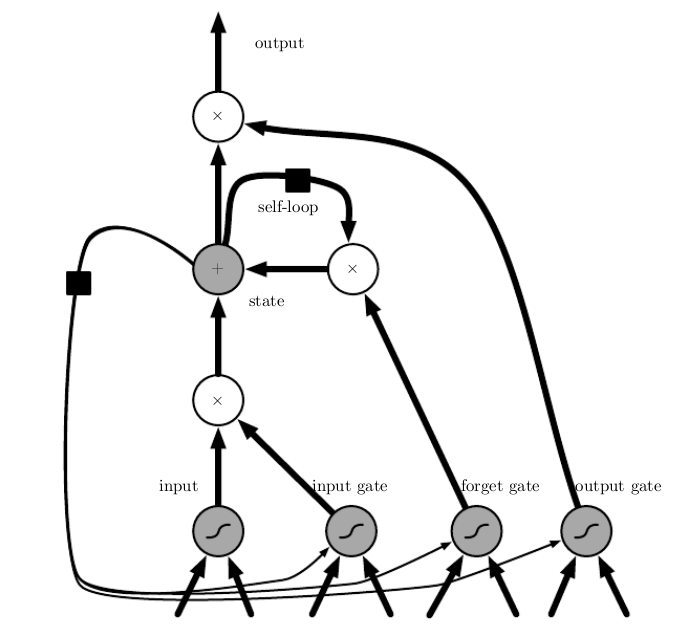
\includegraphics[width=10cm]{figuras/lstm.png}
    \fonte{\cite{graves}}
  \end{varwidth}
\end{figure}

\subsection{\textit{Bidirectional Long Short-Term Memory}} \label{sec:bilstm}

A ideia de adicionar camadas em direções opostas nas RNNs foi proposta por \textcite{Schuster}, sendo denominadas redes bidirecionais.
Essa técnica, posteriormente, foi adaptada nos estudos de \textcite{bilstm}, que propuseram uma LSTM Bidirecional, ou \textit{Bidirectional Long Short-Term Memory} (biLSTM).
Sua estrutura é formada por duas LSTMs: 
uma recebendo as entradas à frente, enquanto outra as recebe na direção oposta.
O intuito é que a saída de cada unidade influencie indiretamente em sua contraparte, de forma que os gradientes não dispersem conforme o tempo.


\subsection{\textit{Gated Recurrent Unit}} \label{sec:gru}
A \textit{Gated Recurrent Unit} (GRU) é um tipo de RNN introduzida por \textcite{Cho}.
Sua estrutura é semelhante às das LSTMs, mas têm uma arquitetura minimalista e, portanto, são computacionalmente mais eficientes. 
Utilizam dois tipos principais de portas (\textit{gates}) para controlar o fluxo de informações dentro da unidade: a porta do esquecimento (\textit{Reset gate}) e a porta de atualização (\textit{update gate}).

\begin{figure}[!htb] \centering
  \caption{Estrutura de uma GRU} \label{figura:gru}
  \begin{varwidth}{\linewidth}
    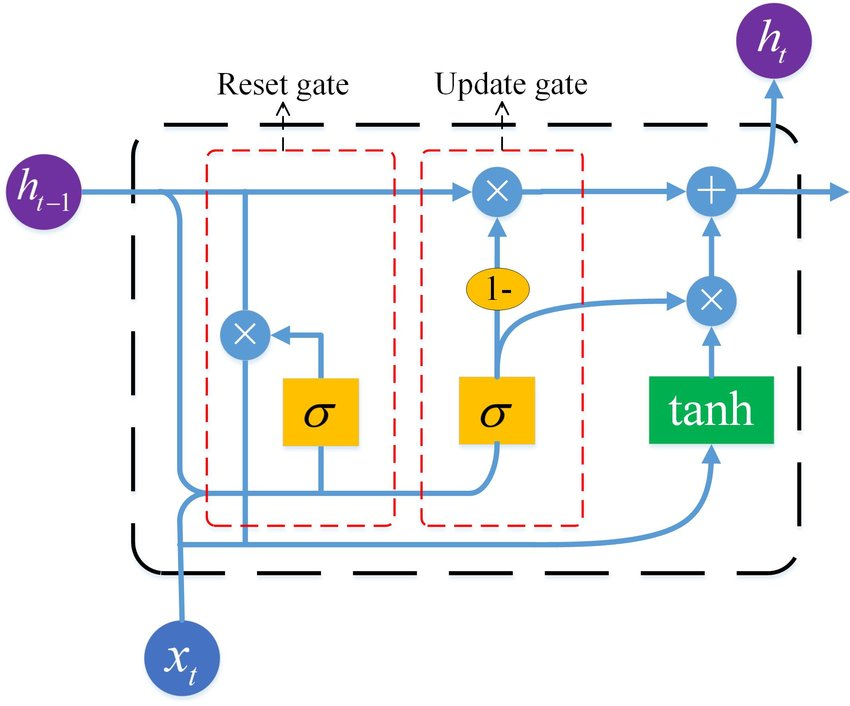
\includegraphics[width=10cm]{figuras/gru.png}
    \fonte{\cite{gru-image}}
  \end{varwidth}
\end{figure}

\section{\textit{Séries temporais}} \label{sec:temp}
Séries temporais são conjuntos de dados intrinsecamente relacionados ao tempo; sua natureza ordenada e agrupada em intervalos regulares
torna a sequência cronológica fundamental \cite{Esling}. Alguns desses conjuntos possuem ciclos repetitivos em períodos distintos, chamados sazonalidades. 
Possuem inúmeras aplicações, representando vendas, preços de ações e variações nos mais diversos contextos.

O número de amostras e a correlação de eventos são fatores primordiais que definem a complexidade da análise.
\textcite{Nison} destaca que, já no século XVIII, os japoneses desenvolveram uma forma de
visualização de séries temporais popularmente conhecida como \textit{Candlestick}.

%Desde então, o comportamento que denota sua variação, representada em ativos como no mercado financeiro, intriga economistas, estastísticos e professores de finanças \cite{Fama}

%\subsection{Previsão de preços} \label{sec:previsao}

%Prever preços não é algo necessariamente novo ou exclusivo de mercados digitais. Porém, utilizar os recursos computacionais atuais aliados a técnicas especificas para séries temporais podem proporcionar uma maior assertividade.

\section{Estado da arte} \label{sec:estado}

\textcite{Fer} obtiveram sucesso em prever preços do Bitcoin para o dia seguinte com modelos LSTM. Autores como \textcite{Tri} combinam métodos bayesianos, processamento de sinais e redes neurais a fim de prever o preço desses ativos em múltiplos intervalos de tempo.
Estudos propostos por \textcite{lstmvsgru} comparam o desempenho de LSTMs e GRUs na previsão de preços de criptomoedas no gráfico diário com janelamento de 32 dias.
\textcite{Siami} propuseram uma pesquisa comparativa entre LSTMs e BiLSTMs no contexto de séries temporais como um todo, enquanto
\textcite{Zhang} compilaram resultados de modelos para previsão de preço, detecção de bolha e construção de portfólio que podem aumentar a lucratividade no âmbito das criptomoedas.

A variedade de algoritmos empregados e a diversidade em resultados obtidos demonstram a complexidade do problema, reforçando, assim, a necessidade de se explorar diferentes abordagens. A Tabela \ref{tabela:lista_estudos} apresenta uma comparação entre os estudos citados e o presente trabalho.

\begin{table}[!htb]
  \scriptsize
  \caption{Comparação entre estudos na área} \label{tabela:lista_estudos}
  \begin{tabularx}{\textwidth}{l|X|X|X|X|X} \hline
    Pesquisadores & Ativo & Entradas & Saídas & Modelos & Métricas \\ \hline
    \cite{lstmvsgru} & Bitcoin & Preço & Preço médio & LSTM, GRU & SMAPE \\ \hline
    \cite{Fer} & Bitcoin & Preço & Preço & LSTM & RMSE \\ \hline
    \cite{Siami} & Ações & Preço & Preço& ARIMA, LSTM, BiLSTM & RMSE \\ \hline
    \cite{Tri} & Bitcoin & Preço ou indicadores& Preço & DANN, LSTM, BiLSTM, CNN-BiLSTM & RMSE, MAE, MAPE \\ \hline
    Autor & Bitcoin & Preço, trocas e volume & Preço & ARIMA, LSTM, BiLSTM e GRU & MAPE, RMSE, $R^2$ \\ \hline
  \end{tabularx}
  \fonte{Elaborado pelo autor, 2024.}
\end{table}
